\documentclass[11pt,a4paper]{scrartcl}
\typearea{12}
\usepackage{graphicx}
\usepackage{pstricks}
\usepackage{amsmath}
\begin{document}


\section*{An introduction to programming}

To save time learning syntax we are going to look at a block
programming language where the commands appear as block. When you get
used to a programming language typing is, of course, quicker than
moving blocks around, but block programming languages are very
convenient; this programming environment is hosted online which is
even more convenient since it means we don't have to install
anything. The site an be found at \texttt{snap.berkeley.edu}.

Here is a simple programme for drawing a square; we will start with
this and try to make more complicated drawings.
\begin{center}
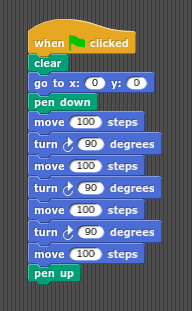
\includegraphics{basic_square.png}
\end{center}
Enter this and make sure it draws a square! One thing about this
program is that after it draws the square the arrow ends up pointing a
different direction to the direction it started in; can you fix this?

Now, the annoying thing about this programme is having to move over
the same two commands again and again; this isn't just a problem
because it is boring, it also disguises the main point of the program,
doing the same thing four times. Programmes are best when they are easy to interpret, so here we can make the programme simpler using a repeat:
\begin{center}
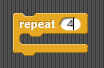
\includegraphics{repeat.png}
\end{center}
Can you use that to make the programme more succinct and readable? 

Now, look at this programme
\begin{center}
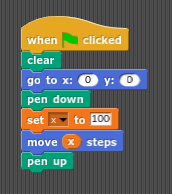
\includegraphics{variable.png}
\end{center}
Instead of writing directly that it is to go 100 steps and make a
\textsl{variable} called \texttt{x} and tell it to go \texttt{x}
steps. This is kind of pointless in this short program but we will see
soon how useful variables are. Do the same to your square programme!
You will need to click the \lq{}Make a variable\rq{} button to add a
variable; add it for all sprites, we'll only be using one sprite at a
time in this class.
\end{document}
